\documentclass[a4paper,11pt]{article}

%-----------------------------------------

\usepackage[utf8]{inputenc} %Wegen Umlaute
\usepackage[ngerman]{babel} %Wegen Umlaute
\usepackage[T1]{fontenc} %pdf umlaute gefunden
\usepackage{graphicx}
%\usepackage{hyperref}
%\usepackage{floatflt,epsfig} 
\usepackage{float}%für bilder und grafiken
\usepackage{listings}
\lstset{language=VHDL, basicstyle=\small \ttfamily,  showtabs=false, keywordstyle=\bfseries, 
showstringspaces=false, framexleftmargin= 8mm, framexrightmargin= 15.4mm, frame=single, numbers=left, numberstyle=\tiny, stepnumber=1}
\usepackage{amsmath,bm}
\usepackage{chngcntr} %Abbildungsnummer 
\usepackage{caption}
\usepackage[absolute]{textpos}
\usepackage{courier}

%-----------------------------------------


\begin{document}


%\maketitle
\begin{titlepage}

\begin{textblock*}{70mm}(120mm,20mm)
    
\includegraphics[width=232px,height=46px]{HSFuldaLogo.pdf}
    \end{textblock*}

    \begin{center}
    \huge \textbf{\textsf{FD-Netzwerk}} \\
    \vspace{0.5cm}

\begin{figure}[H]
\centering
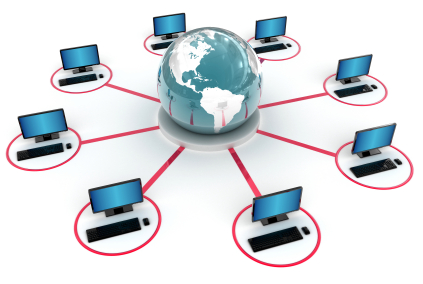
\includegraphics[width=0.4\textwidth]{network.jpg}
\numberwithin{figure}{section}
%\caption{Netzwerk}
\end{figure}
$~~$\\


    \normalsize
    vorgelegt am: \today \\
    \vspace{0.5cm}
    \large \textbf{Fachbereich~Angewandte Informatik \\Hochschule~Fulda}\\
    \vspace{0.5cm}
    \huge \textbf{Planung und Durchführung vom Netzwerkprojekt}\\
    \vspace{0.5cm}
    \large \textbf{Prof. Dr.-Ing Anatol Badach}\\
    \vspace{0.5cm}
    \large{SS16}
    \vspace{0.5cm}
    \end{center}
 \normalsize{
    \begin{tabular}{ll}
    	Name: & {Hakan Cihan} \\
    	%Matrikelnummer: & {431746} \\
    	Email: & {hakan.cihan@informatik.hs-fulda.de} \\
    	\\
    	Name: & {Kevin Klüber} \\
    	%Matrikelnummer: & {134880} \\
    	Email: & {kevin.klueber@informatik.hs-fulda.de} \\
    	\\
    	Name: & {Marvin Klüber} \\
    	%Matrikelnummer: & {132243} \\
    	Email: & {marvin.klueber@informatik.hs-fulda.de} \\
	\\
    	Name: & {Jakob Stockmayer} \\
    	%Matrikelnummer: & {239792} \\
    	Email: & {jakob.stockmayer@informatik.hs-fulda.de} \\
	\\
    	Name: & {Lukas Wegstein} \\
    	%Matrikelnummer: & {139018} \\
    	Email: & {lukas.wegstein@informatik.hs-fulda.de} \\
	 \\
    	
    \end{tabular}\\
    }
\end{titlepage}
\newpage
\tableofcontents
\newpage
\makeatletter
\renewcommand{\l@figure}{\@dottedtocline{1}{0cm}{1.2cm}}
\makeatother
\listoffigures
\newpage

\section{Thema 1}


\section{Thema 2}
\subsection{Subsection 1}




\end{document}